\documentclass{ohm_project_description}

\projecttitle{Robocup@Home (Autonomous Service Robot)}
\projectauthor{Labor für mobile Robotik}
\projectdate{2026}

\begin{document}

\maketitle
\thispagestyle{fancy}

\vspace*{-2.5cm}
\begin{figure}[h!]
    \centering
    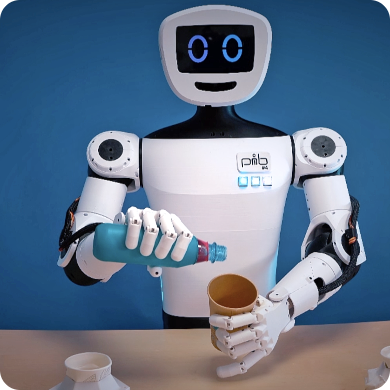
\includegraphics[height=4cm]{img/pib-pours-a-drink.png}
\end{figure} 


This project proposal lists various potential project topics for a humanoid service robot and the Robocup@Home League. The specific topic will be determined in consultation with the supervisor, based on the interests and skills of the students. Students are asked to contribute to the lab's Robocup@Home team. \\

General information on the @Home competition and rules can be found here: \url{https://athome.robocup.org/}.\\

Possible topics include, but are not limited to:

\begin{itemize}[leftmargin=0.5cm]
    \setlength\itemsep{.5em}
    \item \textbf{Topic 1: Perception for an autonomous service robot} \\
        Develop and expand the robot's perception pipeline for navigation, object detection and manipulation. Explore and integrate the use of state-of-the-art robotic foundation models such
        as Nvidia Cosmo3 (\url{https://arxiv.org/abs/2606.02800}).

    \item \textbf{Topic 2: Safety concept for an autonomous service robot} \\
        Implement a wholistic safety concept (hardware+software) that enables the robot to safely operate in a collaborative environment (\textit{CoBot}) while making sure not to harm persons or causing damage.

    \item \textbf{Topic 3: User interaction (UX/UI) for an autonomous service robot} \\
        Develop, implement and evaluate a user interaction (UX/UI) concept that allows the robot to be operated by laypersons. The robot should be easily controllable by voice or gesture commands and clearly communicate its current state and intended actions. 

\end{itemize}

\textbf{In case you are interested in working on the robot, but not in the listed topics, feel free to contact us nontheless. We might find another topic that suits you!}


\vspace{0.5cm}
These topics can be pursued as a Bachelor's or Master's thesis or as a project work for two to three students.


\vfill
\textcolor{ohm_red}{\rule{\linewidth}{0.4mm}}
\textbf{\textcolor{ohm_red}{Labor für mobile Robotik}} \\
\begin{tabular}{@{}ll}
\textbf{Supervisor:} & Prof. Dr. Enrico Schröder \\
\textbf{E-Mail:}   & \href{mailto:enrico.schroeder@th-nuernberg.de}{enrico.schroeder@th-nuernberg.de} \\
\end{tabular}

\end{document}